\documentclass{ximera}
\title{Graphics and interactives}
\author{Bart Snapp and Jason Nowell}
\begin{document}
\begin{abstract}
    How to include graphics and other interactive content.
\end{abstract}
\maketitle



\section{Including images}

The preferred way to include graphics is with TikZ.
\begin{image}
  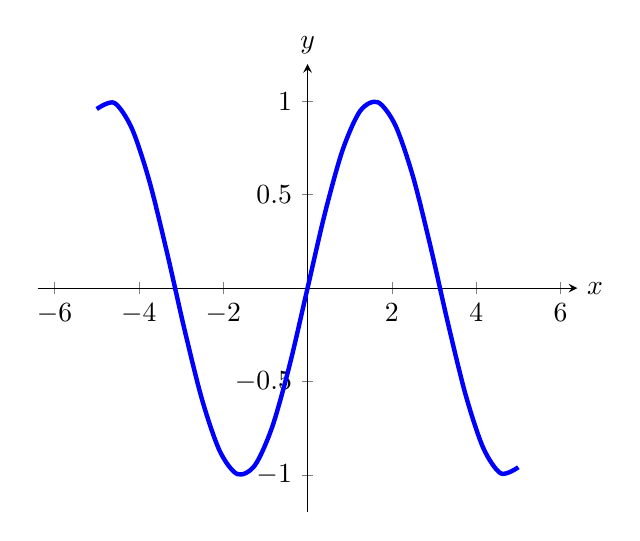
\begin{tikzpicture}
    \begin{axis}[
        xmin=-6.4,
        xmax=6.4,
        ymin=-1.2,
        ymax=1.2,
        axis lines=center,
        xlabel=$x$,
        ylabel=$y$,
        every axis y label/.style={at=(current axis.above origin),anchor=south},
        every axis x label/.style={at=(current axis.right of origin),anchor=west},
      ]
      \addplot [ultra thick, blue, smooth] {sin(deg(x))};
    \end{axis}
  \end{tikzpicture}
\end{image}

\begin{verbatim}
\begin{image}
  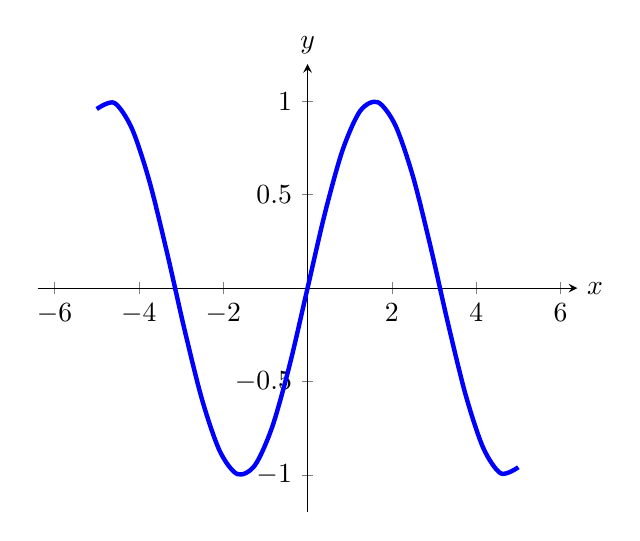
\begin{tikzpicture}
    \begin{axis}[
        xmin=-6.4,
        xmax=6.4,
        ymin=-1.2,
        ymax=1.2,
        axis lines=center,
        xlabel=$x$,
        ylabel=$y$,
        every axis y label/.style={at=(current axis.above origin),anchor=south},
        every axis x label/.style={at=(current axis.right of origin),anchor=west},
      ]
      \addplot [ultra thick, blue, smooth] {sin(deg(x))};
    \end{axis}
  \end{tikzpicture}
\end{image}
\end{verbatim}


Another method is to use \verb|\includegraphics|. Here we see an included a JPEG and a PNG:

\begin{verbatim}
\begin{image}
  
\includegraphics[width=.3\textwidth]{missionPatch.jpg}\qquad
%% chimera.png is licensed under the Creative Commons Attribution-Share 
%% Alike 3.0 Unported license.
%% Attribution: I, Sailko
%% https://commons.wikimedia.org/wiki/File:Chimera_d%27arezzo,_fi,_04.JPG
  
\includegraphics[width=\textwidth]{chimera.png}
\end{image}
\end{verbatim}
In the code above, the command image is just a Ximera provided wrapper
that can be redefined for printing. It does automatically resize
content though and can be useful for showing images side-by-side:
\begin{image}
  
  
\includegraphics[width=2in\textwidth]{missionPatch.jpg}\qquad
%% chimera.png is licensed under the Creative Commons Attribution-Share 
%% Alike 3.0 Unported license.
%% Attribution: I, Sailko
%% https://commons.wikimedia.org/wiki/File:Chimera_d%27arezzo,_fi,_04.JPG
  
\includegraphics[width=.3\textwidth]{chimera.png}
\end{image}

Here we have a pdf
\begin{center}
  
\includegraphics{llama.pdf}
\end{center}


\section{Videos}

We can embed YouTube Videos with 




\verb|\youtube{FvgF95i0_lw}| which would embed the video into the page, like this:
\begin{center}
        \youtube{FvgF95i0_lw}
\end{center}



\section{The graph command}

The easiest way to include an interactive graph is to use the
\verb|\graph| command. Unfortunately, the \verb|\graph| command
doesn't draw a graph in the PDF, rather, it states (in words) that a
graph is produced.
\[
\graph{x^2}
\]
There are a number of options for the \verb|\graph| command:


\paragraph{Change viewing window}
\begin{verbatim}
\[
\graph[xmin=-5,xmax=5,ymin=-5,ymax=5]{y=x^2}
\]
\end{verbatim}



\paragraph{Restricting domain}


\begin{verbatim}
\[
\graph{x^2 \left\{ 1 \leq x \leq 10 \right\} }
\]
\end{verbatim}
\paragraph{Default panel displayed}

  
\begin{verbatim}
\[
\graph[panel]{x^2}
\]
\end{verbatim}
\paragraph{Restricting window}

  
\begin{verbatim}
\[
\graph[xmin=0, xmax=10, ymin=0, ymax=10]{x^2}
\]
\end{verbatim}
\paragraph{Axis labels}

  
\begin{verbatim}
\[
\graph[xAxisLabel="time", yAxisLabel="distance"]{y=x}
\]
\end{verbatim}
\paragraph{Hide axes}

  
\begin{verbatim}
\[
\graph[hideXAxis=true, hideYAxis=true]{x^2}
\]
\end{verbatim}
\paragraph{Hide tick marks}

  
\begin{verbatim}
\[
\graph[hideXAxisNumbers=true, hideYAxisNumbers=true]{x=y^2}
\]
\end{verbatim}
\paragraph{Polar graphing}

  
\begin{verbatim}
\[
\graph{r=\theta}
\]
\end{verbatim}
\paragraph{Polar gridlines}


\begin{verbatim}
\[
\graph[polar]{y=x^2}
\]
\end{verbatim}
\paragraph{Graphing a piecewise function}


\begin{verbatim}
\[
\graph{ \sin(x)\left\{x<0\right\}, 2x\left\{ x>=0 \right\} }
\]
\end{verbatim}


\section{Desmos}

If you require further features from
\link[Desmos]{https://www.desmos.com/}, you can sign up for an account
and include your worksheets like this:

\begin{verbatim}
\begin{center}
\desmos{zwywds7med}{800}{600}
\end{center}
\end{verbatim}
\begin{center}
\desmos{zwywds7med}{800}{600}
\end{center}


  \section{How to embed GeoGebra}

        You can also use \link[GeoGebra]{https://www.geogebra.org/}. Embed the
        widget using the syntax \verb|\geogebra{ID}{width}{height}|, where ID
        is the widget ID and width and height are the dimensions (in pixels)
        you want the embedded widget to have.
        
    
        \begin{center}
            \geogebra{XC3FXUdJ}{800}{600}%%https://www.geogebra.org/m/XC3FXUdJ
        \end{center}
        
        The above embedding is generated via the code:
        
        \begin{verbatim}
            \begin{center}
            \geogebra{XC3FXUdJ}{800}{600}
            \end{center}
        \end{verbatim}      

        \section{How to embed Desmos 3D}

        \begin{center}
          \desmosThreeD{bb4exrhrl3}{800}{600}
        \end{center}
        \begin{verbatim}
          \begin{center}
          \desmosThreeD{bb4exrhrl3}{800}{600}
          \end{center}
      \end{verbatim}    
      






\end{document}
